\section{Quantization and Obstruction}\label{sec:qo}
In the \nameref{sec:bv}, we had the data of an $\infty$-dimensional $(-1)$-symplectic geometry $(\cE,Q,\omega)$ that describe the QFT.
Recall the classical data: the space of \textbf{local functionals}, $\sO_{loc}(\cE)\subset \sO(\cE)$, in which the classical interaction $I_0=\int_X \cL$ is an element of $\sO_{loc}(\cE)$. $I_0$ solves the CME, $QI_0+\hf \lcb I_0,I_0\rcb_0=0$. Here $\lcb -,-\rcb_0$ is the BV bracket with respect to the BV kernel $K_0=\omega^{-1}$ and is well-defined on $\sO_{loc}(\cE)$. However the BV operator $\Delta_0$ is ill-defined on $\sO_{loc}(\cE)$ and $\sO(\cE)$, implying that the naive QME $QI_0+\hbar \Delta_0 I_0+\hf \lcb I_0,I_0\rcb=0$ does not make sense.

One way out of this problem is to use regularization to define an effective QME. We defined the Poisson kernel $K_0=K_r+QP_r$, where $K_r$ is smooth, leading to a well-defined BV operator $\Delta_r$ on $\sO(\cE)$. For each $r$, we have constructed $I[r]\in \sO(\cE)$ solving the effective QME
\bea \lb Q+\hbar\Delta_r\rb e^{I[r]/\hbar}=0.\eea
Different regularizations are related by the HRG flow:
\bea e^{I[r']/\hbar}=\exp{\lb \hbar \p_{P^{r'}_r}\rb} e^{I[r]/\hbar}.\eea
We have seen that the effective QME and the HRG are compatible.
\bea 
\tikzset{every picture/.style={line width=0.75pt}}         
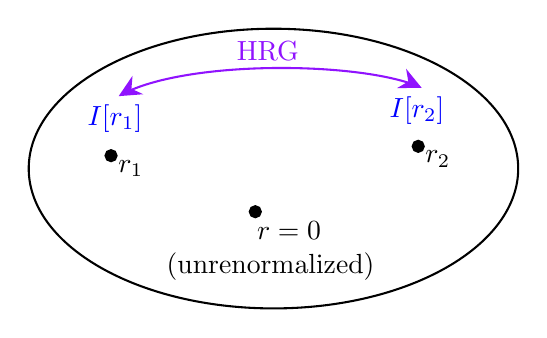
\begin{tikzpicture}[x=0.75pt,y=0.75pt,yscale=-1,xscale=1]


%Curve Lines [id:da944062929767304] 
\draw [color={rgb, 255:red, 144; green, 19; blue, 254 }  ,draw opacity=1 ]   (230.27,95.93) .. controls (262.54,80.07) and (341.87,80.98) .. (370.8,92.41) ;
\draw [shift={(373.33,93.5)}, rotate = 205.15] [fill={rgb, 255:red, 144; green, 19; blue, 254 }  ,fill opacity=1 ][line width=0.08]  [draw opacity=0] (10.72,-5.15) -- (0,0) -- (10.72,5.15) -- (7.12,0) -- cycle    ;
\draw [shift={(227.33,97.5)}, rotate = 329.86] [fill={rgb, 255:red, 144; green, 19; blue, 254 }  ,fill opacity=1 ][line width=0.08]  [draw opacity=0] (10.72,-5.15) -- (0,0) -- (10.72,5.15) -- (7.12,0) -- cycle    ;
%Shape: Circle [id:dp36250985174485173] 
\draw  [fill={rgb, 255:red, 0; green, 0; blue, 0 }  ,fill opacity=1 ] (221,126.17) .. controls (221,124.69) and (222.19,123.5) .. (223.67,123.5) .. controls (225.14,123.5) and (226.33,124.69) .. (226.33,126.17) .. controls (226.33,127.64) and (225.14,128.83) .. (223.67,128.83) .. controls (222.19,128.83) and (221,127.64) .. (221,126.17) -- cycle ;
%Shape: Circle [id:dp6932568334360127] 
\draw  [fill={rgb, 255:red, 0; green, 0; blue, 0 }  ,fill opacity=1 ] (369,121.67) .. controls (369,120.19) and (370.19,119) .. (371.67,119) .. controls (373.14,119) and (374.33,120.19) .. (374.33,121.67) .. controls (374.33,123.14) and (373.14,124.33) .. (371.67,124.33) .. controls (370.19,124.33) and (369,123.14) .. (369,121.67) -- cycle ;
%Shape: Circle [id:dp7842852672394907] 
\draw  [fill={rgb, 255:red, 0; green, 0; blue, 0 }  ,fill opacity=1 ] (290.5,153.17) .. controls (290.5,151.69) and (291.69,150.5) .. (293.17,150.5) .. controls (294.64,150.5) and (295.83,151.69) .. (295.83,153.17) .. controls (295.83,154.64) and (294.64,155.83) .. (293.17,155.83) .. controls (291.69,155.83) and (290.5,154.64) .. (290.5,153.17) -- cycle ;
%Shape: Ellipse [id:dp3283980465228562] 
\draw   (184,132.38) .. controls (184,95.17) and (236.79,65) .. (301.92,65) .. controls (367.04,65) and (419.83,95.17) .. (419.83,132.38) .. controls (419.83,169.59) and (367.04,199.76) .. (301.92,199.76) .. controls (236.79,199.76) and (184,169.59) .. (184,132.38) -- cycle ;

% Text Node
\draw (225.67,126.9) node [anchor=north west][inner sep=0.75pt]    {$r_{1}$};
% Text Node
\draw (373.67,122.4) node [anchor=north west][inner sep=0.75pt]    {$r_{2}$};
% Text Node
\draw (292.5,156.57) node [anchor=north west][inner sep=0.75pt]    {$r=0$};
% Text Node
\draw (210.87,100.18) node [anchor=north west][inner sep=0.75pt]  [color={rgb, 255:red, 0; green, 0; blue, 255 }  ,opacity=1 ]  {$I[ r_{1}]$};
% Text Node
\draw (356.42,96.3) node [anchor=north west][inner sep=0.75pt]  [color={rgb, 255:red, 0; green, 0; blue, 255 }  ,opacity=1 ]  {$I[ r_{2}]$};
% Text Node
\draw (282.77,69.83) node [anchor=north west][inner sep=0.75pt]  [color={rgb, 255:red, 144; green, 19; blue, 254 }  ,opacity=1 ] [align=left] {HRG};
% Text Node
\draw (249,171.5) node [anchor=north west][inner sep=0.75pt]   [align=left] {(unrenormalized)};
\end{tikzpicture}
\eea


\subsection{Heat kernel regularization}\label{subsec:hker}
In physics, there are many ways of regularizations. One regularization method that connects to geometry is the heat kernel regularization. Typically, fixing a choice of metric, we have 
\begin{itemize}
    \item the adjoint of the elliptic operator $Q:\cE\to \cE$, denoted as $Q^\dagger: \cE\to \cE$,
    \item a generalized Laplacian, $\lsb Q,Q^\dagger\rsb= QQ^\dagger+Q^\dagger Q$.
\end{itemize}
Thus we can define a heat operator $e^{-L\lsb Q,Q^\dagger\rsb}$ for $L>0$. Let $K_L\in \sym^2(\cE)$ be the kernel of the heat operator by 
\bea \lb e^{-L\lsb Q,Q^\dagger\rsb}\alpha\rb \lb x\rb
=\int dy \lan K_L(x,y),\alpha(y)\ran\quad \text{for }\alpha\in\cE.\eea 
Here $\lan-,-\ran$ is the pairing from $\omega$.
Note that
\begin{itemize}
    \item $K_0=\lim_{L\to 0} K_L$ is the $\delta$-function distribution $\omega^{-1}$,
    \item $K_L\in \sym^2(\cE)$ is smooth for $L>0$.
\end{itemize}

Let $P_L$ be the kernel of the operator $\int_0^L dt\ Q^\dagger e^{-t\lsb Q,Q^\dagger\rsb} $. Explicitly, we have 
\bea P_L= \int_0^L dt \lb Q^\dagger \otimes 1\rb K_t.\eea
The operator equation 
\bea \lsb Q, \int_0^L dt\ Q^\dagger e^{-t\lsb Q,Q^\dagger\rsb} \rsb 
= \int_0^L dt \lsb Q,Q^\dagger\rsb e^{-t\lsb Q,Q^\dagger\rsb} 
=1-e^{-L\lsb Q,Q^\dagger\rsb}\eea
can be translated into the kernel equation:
\bea K_0-K_L=(Q\otimes 1+1\otimes Q)P_L\eea
or simply written as
\bea K_0-K_L=Q \lb P_L\rb.\eea
We can use $K_L$ to define the effective QME. 

For $0<\varepsilon<L$, similarly the operator equation is 
\bea \lsb Q, \int_\varepsilon^L dt\ Q^\dagger e^{-t\lsb Q,Q^\dagger\rsb} \rsb 
=e^{-\varepsilon\lsb Q,Q^\dagger\rsb}-e^{-L\lsb Q,Q^\dagger\rsb}\eea
or 
\bea K_\varepsilon-K_L=(Q\otimes 1+1\otimes Q)P_\varepsilon^L,\eea
where $P^L_\varepsilon= \int_\varepsilon^L dt \lb Q^\dagger \otimes 1\rb K_t$ is called the \emph{regularized propagator}. 
Now we can use $P^L_\varepsilon$ to connect the effective QME at $\varepsilon$ with the effective QME at $L$ via the HRG, $\exp{\lb \hbar\p_{P_\varepsilon^L}\rb}$.
\begin{rmk}
$P_0^\infty= \int_0^\infty dt \lb Q^\dagger \otimes 1\rb K_t$ is the \emph{full propagator}. At $t=0$, one will encounter ultraviolet (UV) divergence since there exists a singularity for the full propagator. On a non-compact manifold, one will encounter infrared (IR) divergence at $t=\infty$.
\end{rmk}


\subsection{Constructing effective BV quantization using heat kernel regularization}
\paragraph{Step 1: The method of counter-term.}
Let $I_0\in \sO_{loc}(\cE)$ be the classical interaction. Since $P_0^L$ is singular, the limit $\lim_{\varepsilon\to 0} \exp{\lb \hbar\p_{P_\varepsilon^L}\rb} e^{I_0/\hbar}$ does not exist. Pictorially, all the loop diagrams:
\bea 
    \begin{fmffile}{fddlim}
    \begin{tabular}{c}
        \begin{fmfgraph*}(150,80)
                \fmfleft{i1,i2}
                \fmfright{o1,o2}
                \fmf{plain,tension=4}{i1,v1}
                \fmf{plain,tension=4}{i2,v1}
                \fmf{plain,tension=4}{v2,o1}
                \fmf{plain,tension=4}{v2,o2}

                \fmf{plain,left=1,tension=0.4,label=$P_\varepsilon^L$,label.side=left}{v1,v2}
                \fmf{plain,left=0.5,tension=0.8}{v1,v2}
                \fmf{phantom,right=0.2,tension=2,label=$\cdot$,label.side=left}{v1,v2}
                \fmf{phantom,right=0.5,tension=0.8,label=$\cdot$,label.side=left}{v1,v2}
                \fmf{phantom,right=0.8,tension=0.6,label=$\cdot$,label.side=left}{v1,v2}
                \fmf{plain,right=1,tension=0.4,label=$P_\varepsilon^L$,label.side=right}{v1,v2}
                \fmfv{label=$I_0$,label.angle=170,decor.shape=circle,decor.filled=full,decor.size=2thick}{v1}
                \fmfv{label=$I_0$,label.angle=10,decor.shape=circle,decor.filled=full,decor.size=2thick}{v2}
        \end{fmfgraph*}
        \end{tabular}
    \end{fmffile}\\
\eea
are divergent as $\varepsilon\to 0$.

To cancel the divergences, one can find the \emph{counter-terms}, $I^\epsilon\in \hbar \sO_{loc}(\cE)[[ \hbar]]$, which are $\varepsilon$-dependent and singular as $\varepsilon\to 0$ such that
\bea \lim_{\varepsilon\to 0} \exp{\lb \hbar\p_{P_\varepsilon^L}\rb} e^{\lb I_0+I^\epsilon\rb/\hbar}\coloneqq e^{I[L]^{naive}/\hbar}\eea exists. 
Such defined $I[L]^{naive}$ has the following advantage: for $0<L_1<L_2$, 
\bea e^{I[L_2]^{naive}/\hbar}
&= \lim_{\varepsilon\to 0} \exp{\lb \hbar\p_{P_\varepsilon^{L_2}}\rb} e^{\lb I_0+I^\epsilon\rb/\hbar}\\
&= \lim_{\varepsilon\to 0} \exp{\lb \hbar\p_{P_{L_1}^{L_2}}\rb} \exp{\lb \hbar\p_{P_\varepsilon^{L_1}}\rb} e^{\lb I_0+I^\epsilon\rb/\hbar} \quad \text{using } P_\varepsilon^{L_2}=P_{L_1}^{L_2}+P_\varepsilon^{L_1}\\
&= \exp{\lb \hbar\p_{P_{L_1}^{L_2}}\rb} \lim_{\varepsilon\to 0} \exp{\lb \hbar\p_{P_\varepsilon^{L_1}}\rb} e^{\lb I_0+I^\epsilon\rb/\hbar} \quad \text{since } P_{L_1}^{L_2} \text{ is smooth}\\
&= \exp{\lb \hbar\p_{P_{L_1}^{L_2}}\rb} e^{I[L_1]^{naive}/\hbar}.
\eea
In other words, the family $\lcb I[L]^{naive}\rcb_{L>0}$ satisfies the HRG flow.
\bea
\tikzset{every picture/.style={line width=0.75pt}} 
\begin{tikzpicture}[x=0.75pt,y=0.75pt,yscale=-1,xscale=1]

%Straight Lines [id:da977711475048066] 
\draw    (10.5,100.67) -- (237.5,100.67) ;
\draw [shift={(240.5,100.67)}, rotate = 180] [fill={rgb, 255:red, 0; green, 0; blue, 0 }  ][line width=0.08]  [draw opacity=0] (10.72,-5.15) -- (0,0) -- (10.72,5.15) -- (7.12,0) -- cycle    ;

% Text Node
\draw (4,78.23) node [anchor=north west][inner sep=0.75pt]    {$0$};
% Text Node
\draw (3.12,96) node [anchor=north west][inner sep=0.75pt]  [font=\normalsize,rotate=-0.88]  {$\blt$};
% Text Node
\draw (58,96) node [anchor=north west][inner sep=0.75pt]  [font=\normalsize,rotate=-0.88]  {$\blt$};
% Text Node
\draw (166.12,96) node [anchor=north west][inner sep=0.75pt]  [font=\normalsize,rotate=-0.88]  {$\blt$};
% Text Node
\draw (58,77.23) node [anchor=north west][inner sep=0.75pt]    {$L_{1}$};
% Text Node
\draw (165.5,76.23) node [anchor=north west][inner sep=0.75pt]    {$L_{2}$};
% Text Node
\draw (245.5,93.07) node [anchor=north west][inner sep=0.75pt]    {$L$};
% Text Node
\draw (40.5,108.07) node [anchor=north west][inner sep=0.75pt]    {$I[L_{1}]^{naive}$};
% Text Node
\draw (152.5,108.07) node [anchor=north west][inner sep=0.75pt]    {$I[L_{2}]^{naive}$};
% Text Node
\draw (110,106.57) node [anchor=north west][inner sep=0.75pt]    {$\overset{\text{HRG}}{\leadsto}$};
\end{tikzpicture}
\eea
However, $\lcb I[L]^{naive}\rcb_{L>0}$ may NOT satisfy the QME!

\paragraph{Step 2: Further corrections.}
Adjust $I^\epsilon$ to $\Tilde{I}^\epsilon$ by finding further corrections such that
\bea e^{I[L]/\hbar}
&= \lim_{\varepsilon\to 0} \exp{\lb \hbar\p_{P_\varepsilon^{L}}\rb} e^{\lb I_0+\Tilde{I}^\epsilon\rb/\hbar}\eea
and the defined limit $I[L]$ satisfies the QME.

\begin{rmk}
Step 1 is always possible.
Step 2 is NOT always possible; it might have \emph{obstructions}, in physics this is called the \emph{gauge anomaly}.
\end{rmk}

\begin{rmk}
There are cases where $\varepsilon$-dependent counter-terms are not required in the sense that the limit 
\bea e^{I[L]/\hbar}
&= \lim_{\varepsilon\to 0} \exp{\lb \hbar\p_{P_\varepsilon^{L}}\rb} e^{I/\hbar}\eea
exists for a large class of local functionals $I\in \sO_{loc}(\cE)[[\hbar]]$. Such a theory is called \textbf{ultraviolet (UV)-finite}. Then we can explore the meaning of the effective QME, 
\bea \lb Q+\hbar \Delta_L\rb e^{I[L]/\hbar}=0 \quad \text{or }\quad QI[L]+\hbar \Delta_L I[L]+\hf \lcb I[L],I[L]\rcb_L=0.\eea
The upshot is that $L\to 0$ has a meaning in which the effective QME is reduced to $QI+\hf \lsb I,I\rsb=0$, where $\lsb-,-\rsb$ is the \emph{quantum deformed bracket}.
\end{rmk}

In the following sections, we will explain two main UV-finite examples:
\bi[(1)]
\item Chern-Simons type topological theory. In particular, we will discuss the topological quantum mechanics.
\item 2d chiral theory.
\ei

\subsection{Deformation-Obstruction theory}
Let's first consider the quantization problem CME $\leadsto$ QME in a DGBV $\lb \cA,Q,\Delta\rb$. Let $I_0\in \cA_0$ solve the CME, $QI_0+\hf \lcb I_0,I_0\rcb=0$. Our goal is to find 
\bea I=I_0+I_1\hbar+I_2\hbar^2+\cdots \in \cA_0 [[ \hbar]]\eea
solving the QME, $QI+\hbar\Delta I+\hf \lcb I,I \rcb=0$.

\paragraph{Strategy:} find $I_1,I_2,\cdots$ in order of $\hbar$ via
\bea QI+\hbar\Delta I+\hf \lcb I,I \rcb=\cO(\hbar^{n+1})\quad (n\geq 0).\eea 
\begin{itemize}
    \item $n=0$: this is the initial data of CME, $QI_0+\hf \lcb I_0,I_0\rcb=0$.
    \item $n=1$: $\hbar$-term gives $QI_1+\Delta I_0+\lcb I_0,I_1 \rcb=0$. We need to find $I_1$ solving this equation. Let us write it as 
    \bea QI_1+\lcb I_0,I_1 \rcb= -\Delta I_0. \eea
    For convenience, let us denote $\delta=Q+\lcb I_0,-\rcb$. The CME implies that $\delta^2=0$. We need to solve 
    \bea \delta I_1=-\Delta I_0.\eea
    A key observation is that $\delta\lb -\Delta I_0\rb=0$ (exercise). So we see that $-\Delta I_0$ is $\delta$-closed. The solvability of $I_1$ asks whether $-\Delta I_0$ is $\delta$-exact. 
    
    Let $\cO_1=-\Delta I_0$ and let $\lsb \cO_1\rsb\in H^1(\cA,\delta)$ be the corresponding $\delta$-cohomology class. Then
    \begin{prop}
    $I_1$ can be solved $\LRA \lsb \cO_1\rsb=0$ in $H^1(\cA,\delta)$.
    \end{prop}
    Assume $\lsb \cO_1\rsb=0$. Let $I_1$ and $\Tilde{I}_1$ be two solutions. Then
    \bea \delta(I_1-\Tilde{I}_1)=0 \RA \Tilde{I}_1-I_1 \text{ is } \delta-\text{closed}.\eea
    Also, for any $J\in \cA_0$, the solution
    \bea I_1+\delta J \sim I_1,\eea
    where $\sim$ denotes that both sides are gauge equivalent in a suitable sense (i.e. solving a family version of QME along an interval).
    \begin{prop}
    If $I_1$ can be solved, then
    \bea \lcb \text{solution of } I_1\rcb/ \text{gauge}= H^0(\cA,\delta).\eea
    \end{prop}
    
    \item $n>1$: Assume we have found 
    \bea I_{<k}\coloneqq I_0+I_1\hbar +\cdots+I_{k-1} \hbar^{k-1}\eea
    solving \bea QI_{<k}+\hbar\Delta I_{<k}+\hf \lcb I_{<k},I_{<k}\rcb=\cO(\hbar^k).\eea Let's consider the problem of solving $I_k$. The above equation can be written as 
    \bea \lb Q+\hbar\Delta\rb e^{I_{<k}/\hbar}=\cO(\hbar^{k-1})e^{I_{<k}/\hbar}.\eea
    We want to find $I_k$ such that 
    \bea \lb Q+\hbar\Delta\rb e^{\lb I_{<k}+I_k\hbar^k\rb/\hbar}=\cO(\hbar^{k})e^{\lb I_{<k}+I_k\hbar^k\rb/\hbar}.\eea
    Let us write
    \bea \lb Q+\hbar\Delta\rb e^{I_{<k}/\hbar}=\lb \cO_k\hbar^{k-1}+\cO(\hbar^k)\rb e^{I_{<k}/\hbar},\eea
    where $\cO_k$ is the leading term in $\cO(\hbar^{k-1})$.
    Explicitly, we have
    \bea QI_{<k}+\hbar \Delta I_{<k}+\hf \lcb I_{<k},I_{<k}\rcb=\cO_k \hbar^k+\cO(\hbar^{k+1}).\eea
    Similarly, we need to solve
    \bea Q\lb I_{<k}+\hbar^k I_{k}\rb+\hbar \Delta\lb  I_{<k}+\hbar^k I_{k}\rb+\hf \lcb I_{<k}+\hbar^k I_{k}, I_{<k}+\hbar^k I_{k}\rcb= \cO(\hbar^{k+1}).\eea
    This is equivalent to $QI_{k}+\lcb I_{0},I_{k}\rcb=\cO_k$ or $\delta I_{k}=\cO_k$.
    \begin{clm}
    $\cO_k$ is $\delta$-closed.
    \end{clm}
    \begin{sproof}
    Apply $(Q+\hbar\Delta)$ to both sides of
    \bea \lb Q+\hbar\Delta\rb e^{I_{<k}/\hbar}=
    \lb \cO_k \hbar^{k-1}+\cO(\hbar^k)\rb e^{I_{<k}/\hbar}.\eea
    The left-hand side is $\lb Q+\hbar\Delta\rb^2=0$; the leading term on the right-hand side tells us that $Q\cO_k+\lcb I_0,\cO_k\rcb=0$ or $\delta \cO_k=0$. The solvability of $I_k$ asks whether $\cO_k$ is $\delta$-exact.
    \end{sproof}
    \begin{prop}
    Solvability of $I_k \LRA \lsb \cO_k\rsb=0$ in $H^1(\cA,\delta)$. Moreover, if $I_k$ can be solved, then 
    \bea \lcb \text{solution of } I_k\rcb/ \text{gauge}= H^0(\cA,\delta).\eea
    \end{prop}
    \begin{rmk} Terminology.
    \begin{itemize}
        \item $\lsb\cO_k\rsb\in H^1(\cA,\delta)$ is the \textbf{obstruction class} (\textbf{gauge anomaly}) for solving QME up to $\hbar^k$,
        \item $H^1(\cA,\delta)$ is the \textbf{obstruction space},
        \item $H^0(\cA,\delta)$ is the \textbf{tangent space} (or \textbf{deformation space}).
    \end{itemize}
    \end{rmk}
    In particular, we have proved
    \begin{thm}
    If $H^1\lb\cA, Q+\lcb I_0,-\rcb\rb=0$, then there exists a quantization $I=I_0+\hbar I_1+\cdots$ solving the QME, $QI+\hbar\Delta I+\hf \lcb I,I\rcb=0$.
    \end{thm}
\end{itemize}

\subsection{Effective QME}
In the QFT case, things are more complicated since we need to deal with regularization. However, the good thing is that the analogue of deformation-obstruction theory still exists. The relevant complex is $\lb \sO_{loc}\lb \cE\rb, Q+\lcb I_0,-\rcb\rb$. Note that $Q+\lcb I_0,-\rcb$ is well-defined on local functionals and CME implies that $\lb \sO_{loc}\lb \cE\rb, Q+\lcb I_0,-\rcb\rb$ indeed forms a complex.

Similar to the above discussion, we have 
\begin{thm}\label{thm5.2}
The obstruction space for effective BV quantization of $I_0$ is given by
\bea H^1\lb \sO_{loc}\lb \cE\rb, Q+\lcb I_0,-\rcb\rb.\eea
The tangent space (deformation space) is
\bea H^0\lb \sO_{loc}\lb \cE\rb, Q+\lcb I_0,-\rcb\rb.\eea
\end{thm}

\begin{rmk}
The locality is important and allows the computation of the above cohomologies via $\cD$-module methods.
\end{rmk}

\noindent \textsc{Reference}:
Theorem \ref{thm5.2} has many different setups and versions in the literature. The discussion we follow here is 
\cite{costello2011renormalization}, which also contains references for classical works therein.
